\documentclass{article}

\usepackage{tikz}
\usepackage{environ}

\usetikzlibrary{calc,trees,positioning,arrows,chains,shapes.geometric,%
	decorations.pathreplacing,decorations.pathmorphing,shapes,%
	matrix,shapes.symbols,backgrounds,fit,scopes} % required in the preamble
\usepackage{varwidth}

\makeatletter
\newsavebox{\measure@tikzpicture}
\NewEnviron{scaletikzpicturetowidth}[1]{%
	\def\tikz@width{#1}%
	\def\tikzscale{1}\begin{lrbox}{\measure@tikzpicture}%
		\BODY
	\end{lrbox}%
	\pgfmathparse{#1/\wd\measure@tikzpicture}%
	\edef\tikzscale{\pgfmathresult}%
	\BODY
}
\makeatother

\tikzset{
	%Define standard arrow tip
	>=stealth',
	%Define style for boxes
	box/.style={
		rectangle,
		rounded corners,
		dashed,
		draw=black, very thick,
		minimum height=2em,
		text centered,
		execute at begin node={\begin{varwidth}{28em}},
			execute at end node={\end{varwidth}}},
	solidbox/.style={
		rectangle,
		rounded corners,
		draw=black, very thick,
		minimum height=2em,
		text centered,
		execute at begin node={\begin{varwidth}{28em}},
			execute at end node={\end{varwidth}}},
	bigsolidbox/.style={
		rectangle,
		rounded corners,
		draw=black, very thick,
		minimum height=6cm,
		text centered,
		execute at begin node={\begin{varwidth}{28em}},
			execute at end node={\end{varwidth}}},
	% Define arrow style
	fw_arrow/.style={
		->,
		thick,
		shorten <=2pt,
		shorten >=2pt,},
	bw_arrow/.style={
		<-,
		thick,
		shorten <=2pt,
		shorten >=2pt,}
	%	bigbox/.style={blue!50, thick, fill=blue!10, rounded corners, rectangle}
}

\definecolor{mc_gen_color}{RGB}{250,138,31}

\definecolor{det_sim_color}{RGB}{227,66,55}

\definecolor{llh_color}{RGB}{128,0,128}

\tikzstyle{bigboxGeneration} = [draw=mc_gen_color!50, thick, fill=mc_gen_color!20, rounded corners, rectangle]

\tikzstyle{bigboxDetector} = [draw=det_sim_color!50, thick, fill=det_sim_color!20, rounded corners, rectangle]

\tikzstyle{bigboxAnalysis} = [draw=llh_color!50, thick, fill=llh_color!20, rounded corners, rectangle]

\newcommand{\cmark}{\text{\ding{51}}}
\newcommand{\xmark}{\text{\ding{55}}}

\begin{document}

\begin{figure}[htp]
	\resizebox{\textwidth}{!}{
		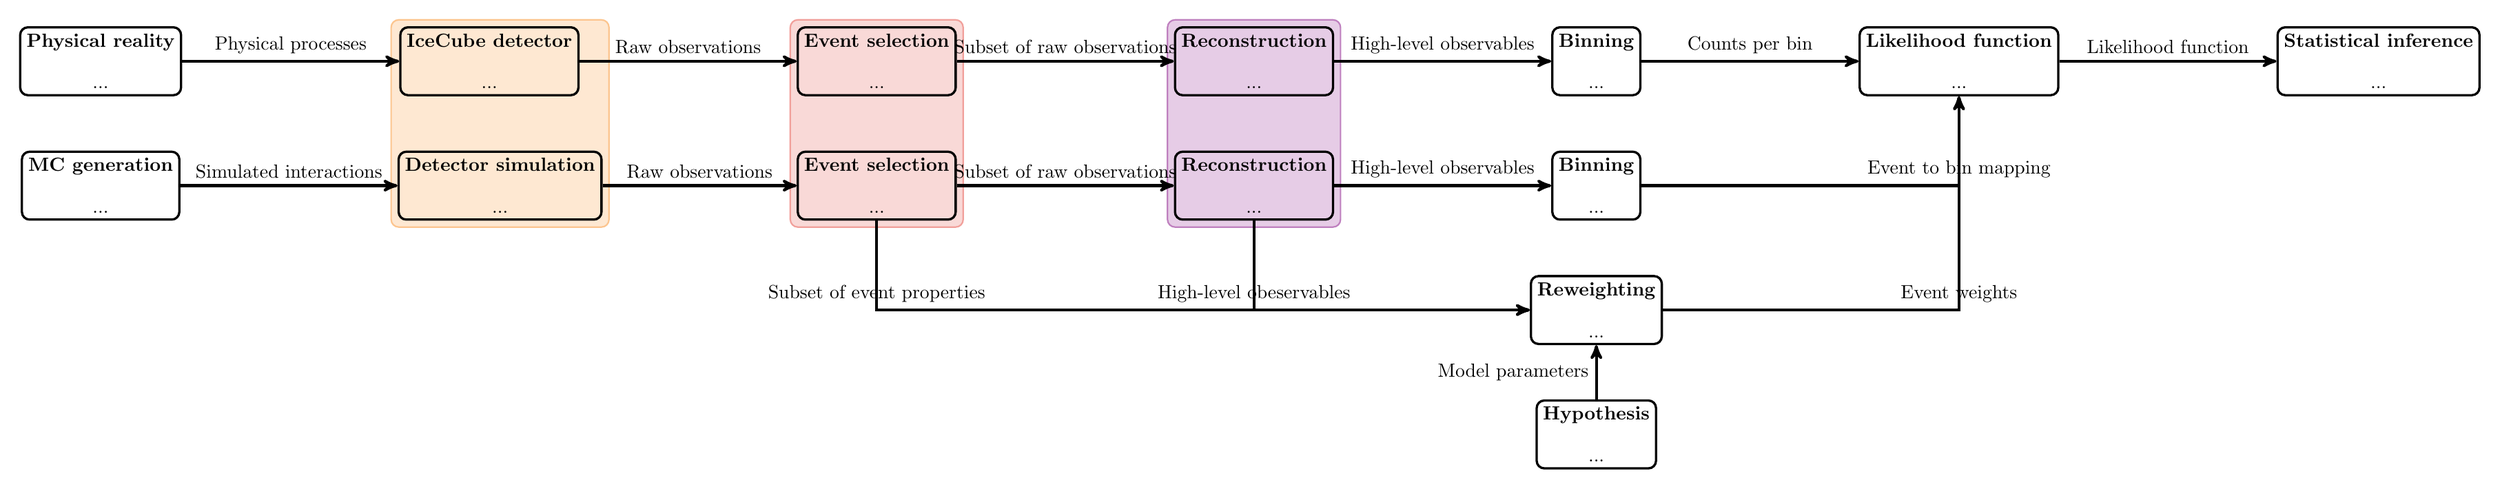
\begin{tikzpicture}[node distance=4cm, auto, start chain]
		
		\node[on chain,solidbox] (reality) {\centering {\bf Physical reality} \\
			\begin{center}
			...
			\end{center}
		};
		
		\begin{scope} [node distance=1cm]
		\node[solidbox, below=of reality] (mc_generation) {\centering {\bf MC generation} \\
			\begin{center}
			...
			\end{center}
		};
		\end{scope}
	
		\node[solidbox, right=of mc_generation] (detector_simulation) {\centering {\bf Detector simulation} \\
			\begin{center}
			...
			\end{center}
		};

		\node[solidbox, right=of reality] (detector) {\centering {\bf IceCube detector} \\
			\begin{center}
			...
			\end{center}
		};
	
		\node[solidbox, right=of detector] (data_selection) {\centering {\bf Event selection} \\
		\begin{center}
		...
		\end{center}
		};
		
		\begin{scope} [node distance=1cm]
		\node[solidbox, below=of data_selection] (mc_selection) {\centering {\bf Event selection} \\
			\begin{center}
			...
			\end{center}
		};
		\end{scope}
	
		\node[solidbox, right=of data_selection] (data_reconstruction) {\centering {\bf Reconstruction} \\
			\begin{center}
			...
			\end{center}
		};
	
		\begin{scope} [node distance=1cm]
		\node[solidbox, below=of data_reconstruction] (mc_reconstruction) {\centering {\bf Reconstruction} \\
			\begin{center}
			...
			\end{center}
		};
		\end{scope}
	
		\node[solidbox, right=of data_reconstruction] (data_binning) {\centering {\bf Binning} \\
			\begin{center}
			...
			\end{center}
		};
	
		\begin{scope} [node distance=1cm]
		\node[solidbox, below=of data_binning] (mc_binning) {\centering {\bf Binning} \\
			\begin{center}
			...
			\end{center}
		};
		\end{scope}
	
		\node[solidbox, right=of data_binning,] (likelihood) {\centering {\bf Likelihood function} \\
			\begin{center}
			...
			\end{center}
		};
	
		\node[solidbox, right=of likelihood] (inference) {\centering {\bf Statistical inference} \\
			\begin{center}
			...
			\end{center}
		};
	
		\begin{scope} [node distance=1cm]
		\node[solidbox, below=of mc_binning] (reweighting) {\centering {\bf Reweighting} \\
			\begin{center}
			...
			\end{center}
		};
	
		\node[solidbox, below=of reweighting] (hypothesis) {\centering {\bf Hypothesis} \\
			\begin{center}
			...
			\end{center}
		};
		\end{scope}
		
		
		%\node[circle, minimum size=1cm, color=black, draw=black, very thick, right=of data_histogram] (likelihood) {\centering {\bf $\mathcal{L}(\vec\theta)$}
		%};
		
		% arrows
		
		%\draw [->,line width=1.5pt] (mc_generation) -- (detector_simulation);
		%\draw [->,line width=1.5pt] (detector_simulation) -- (reweighting);
		%\draw [->,line width=1.5pt] (reweighting) -- (mc_histogram);
		%\draw [->,line width=1.5pt] (mc_histogram) -| (likelihood);
			
		%\draw [->,line width=1.5pt] (data_generation) -- (data_detector_simulation);
		%\draw [->,line width=1.5pt] (data_detector_simulation.east) |- ($(data_detector_simulation.east) + (1.2,0.0)$) |- (data_histogram.west);
		%\draw [->,line width=1.5pt] (data_histogram) -- (likelihood);
		
		\draw [->,line width=1.5pt] (reality) -- (detector) node[midway, above] {Physical processes};
		\draw [->,line width=1.5pt] (detector) -- (data_selection) node[midway, above] {Raw observations};
		\draw [->,line width=1.5pt] (data_selection) -- (data_reconstruction) node[midway, above] {Subset of raw observations};
		\draw [->,line width=1.5pt] (data_reconstruction) -- (data_binning) node[midway, above] {High-level observables};
		\draw [->,line width=1.5pt] (data_binning) -- (likelihood) node[midway, above] {Counts per bin};
		
		\draw [->,line width=1.5pt] (mc_generation) -- (detector_simulation) node[midway, above] {Simulated interactions};
		\draw [->,line width=1.5pt] (detector_simulation) -- (mc_selection) node[midway, above] {Raw observations};
		\draw [->,line width=1.5pt] (mc_selection) -- (mc_reconstruction) node[midway, above] {Subset of raw observations};
		\draw [->,line width=1.5pt] (mc_reconstruction) -- (mc_binning) node[midway, above] {High-level observables};
		\draw [->,line width=1.5pt] (mc_binning) -| (likelihood) node[midway, above] {Event to bin mapping};
		
		\draw [->,line width=1.5pt] (mc_selection) |- (reweighting) node[midway, above] {Subset of event properties};
		\draw [->,line width=1.5pt] (mc_reconstruction) |- (reweighting) node[midway, above] {High-level obeservables};
		\draw [->,line width=1.5pt] (hypothesis) -- (reweighting) node[midway, left] {Model parameters};
		\draw [->,line width=1.5pt] (reweighting) -| (likelihood) node[midway, above] {Event weights};
		\draw [->,line width=1.5pt] (likelihood) -- (inference) node[midway, above] {Likelihood function};
		
		
		% boxes
		
		\begin{pgfonlayer}{background}
		\node[bigboxGeneration] [fit = (detector) (detector_simulation)] {};
		\end{pgfonlayer}
		
		\begin{pgfonlayer}{background}
		\node[bigboxDetector] [fit = (data_selection) (mc_selection)] {};
		\end{pgfonlayer}
		
		\begin{pgfonlayer}{background}
		\node[bigboxAnalysis] [fit = (data_reconstruction) (mc_reconstruction)] {};
		\end{pgfonlayer}
		\end{tikzpicture}
	}% end resize box
	\caption{\textbf{\textit{Diagram of toy experiment steps.}} The three colored boxes indicate the three steps of our toy experiment.
		The left box (almond) summarizes the MC and data generation.
		The center box (salmon) indicates the step in which we apply the detector response.
		The right box (lilac) summarizes the MC reweighting, data and MC histogramming, and final likelihood evaluation from the histograms.
		This final lilac box is repeated for each likelihood evaluation.}
	\label{fig:analysis_overview}
\end{figure}

\begin{figure}[htp]
	\resizebox{\textwidth}{!}{
		\begin{tikzpicture}[node distance=1cm, every node/.style={on chain}, every join/.style={->}]
		\node[on chain, solidbox] (reality) {\centering {\bf Physical reality} \\
			\begin{center}
			...
			\end{center}
		};	
		{ [start branch=mc]
			\node[on chain, solidbox, below=of reality] (mc_generation) {\centering {\bf MC generation} \\
				\begin{center}
				...
				\end{center}
			};
		
			\node[on chain, join, solidbox] (detector_simulation) {\centering {\bf Detector simulation} \\
				\begin{center}
				...
				\end{center}
			};
		
			\node[on chain, join, solidbox] (mc_selection) {\centering {\bf Event selection} \\
				\begin{center}
				...
				\end{center}
			};
			\node[on chain, join=with mc_selection, join=with mc_generation, solidbox] (mc_reconstruction) {\centering {\bf Reconstruction} \\
				\begin{center}
				...
				\end{center}
			};
			\node[on chain, join, solidbox] (mc_binning) {\centering {\bf Binning} \\
				\begin{center}
				...
				\end{center}
			};
		}	
		
		\node[on chain, join, solidbox] (detector) {\centering {\bf IceCube detector} \\
			\begin{center}
			...
			\end{center}
		};
		
		\node[on chain, join, solidbox] (data_selection) {\centering {\bf Event selection} \\
			\begin{center}
			...
			\end{center}
		};
		
		\node[on chain, join, solidbox] (data_reconstruction) {\centering {\bf Reconstruction} \\
			\begin{center}
			...
			\end{center}
		};

		\node[on chain, join, solidbox] (data_binning) {\centering {\bf Binning} \\
			\begin{center}
			...
			\end{center}
		};

		{
		[start branch=weighting]

		\node[on chain, solidbox, join=with mc_selection, join=with mc_reconstruction, below=of mc_binning] (reweighting) {\centering {\bf Reweighting} \\
			\begin{center}
			...
			\end{center}
		};
		}
		
		\node[on chain, join=with chain/mc-end, join=with chain/weighting-end, solidbox] (likelihood) {\centering {\bf Likelihood function} \\
			\begin{center}
			...
			\end{center}
		};
		
		\node[on chain, join, solidbox] (inference) {\centering {\bf Statistical inference} \\
			\begin{center}
			...
			\end{center}
		};
	
		\node[solidbox, below=of reweighting] (hypothesis) {\centering {\bf Hypothesis} \\
			\begin{center}
			...
			\end{center}
		};
		
		\end{tikzpicture}
	}% end resize box
	\caption{\textbf{\textit{Diagram of toy experiment steps.}} The three colored boxes indicate the three steps of our toy experiment.
		The left box (almond) summarizes the MC and data generation.
		The center box (salmon) indicates the step in which we apply the detector response.
		The right box (lilac) summarizes the MC reweighting, data and MC histogramming, and final likelihood evaluation from the histograms.
		This final lilac box is repeated for each likelihood evaluation.}
	\label{fig:analysis_overview2}
\end{figure}

\end{document}